\documentclass[a4paper,11pt]{article}

\usepackage[utf8]{inputenc}
\usepackage[british]{babel}
\usepackage{csquotes}
\usepackage[style=apa]{biblatex}
\usepackage{graphicx}
\usepackage{float}
\usepackage{algorithm}
\usepackage[noend]{algpseudocode}

\def\code#1{\texttt{#1}}

\bibliography{report}

\graphicspath{{images/}}

\title{FIT3036 --- Final Report}
\author{Dylan Pinn --- 24160547 \thanks{dcpin3@student.monash.edu}}
\date{2018, May}
% TODO: Complete title page
% Provide the title, abstract, author names (and contact details,
% affiliations, etc.) and keywords on the first page alone (i.e. this is a
% separate cover page).
% Abstract (<300 words)
% Keywords (<6)

\begin{document}
\maketitle
\vspace{-1ex}
\begin{center}
  % TODO: Update this at the end.
  Word Count: 2299
\end{center}

\begin{abstract}
\end{abstract}
\pagebreak

\tableofcontents
\pagebreak

\section{Introduction}
% TODO: Add starting Introduction

\subsection{Project Objectives}

Our company secured a contract for a local council in Victoria to resurface
roads in a designated square kilometre area. The objectives are to design,
implement, test and deliver a system that will perform these calculations and
display the result to the user.

\subsection{Requirements}

We are to use Google Maps and related products and any satellite/aerial views.
The project involves writing the related code, with an elegant GUI to support
calculations. \autocite[2]{intro:1}

\subsection{Constraints}

We have the following constrains on the project:

\begin{itemize}
  \item Only have access to publicly available data.
  \item Limited to available information online.
  \item No/Limited access to council records.
  \item The project must be finalised by the end of week 12.
\end{itemize}

\section{Background}

The following section introduces the background information of the project,
including project risks, resource requirements and the tasks required to
complete the project and how they were managed.

\subsection{Project Info}

Throughout the project we have been aware of the risks involved. This allows us
to handle them when they do occur and have risk reduction strategies to mitigate
them.

\subsubsection{Project Risks}

We have identified the main project risks and their probability.

\begin{itemize}
  \item Cannot find appropriate road data for calculations. (Medium)
  \item Cannot access data from the OpenStreetMap API.\@ (Low)
  \item Google Maps API offline. (Low)
  \item Problems with infrastructure. (Low)
  \item Completing the project on-time. (Medium)
\end{itemize}

\subsubsection{Risk Reduction Strategies}

Using the following risk reduction strategies we have been able to reduce these
risks and lower their probability.

\begin{itemize}
  \item Research sources for street data from various sources.
    \begin{itemize}
      \item Google Maps did not provide enough data to be useful.
      \item OpenStreetMap provided the required data and an API to access it.
    \end{itemize}
  \item Planning out the project; breaking it up into small components that can
    be worked on sequentially in a short period of time.
\end{itemize}

\subsubsection{Risks Encountered}

The following issues arose throughout the project.

\begin{itemize}
  \item Finding data sources
  \item Finding time to complete the project while working full time and
    completing assessments for other subjects.
\end{itemize}

\subsection{Resource Requirements}

The following hardware and software make up the resources that are required to
complete the project.

\subsubsection{Hardware}

We have decided to use as much Software as a Service (SaaS), Platform as a
Service (PaaS) and Infrastructure as a Service (IaaS) solutions to keep costs
down. \autocite[4]{project-spec:2}

\paragraph{Backend}

To host the backend API, Amazon Web Services (AWS) has been chosen due to its
comprehensive free tier and prior experience with the platform. Integration with
the platform is handled by the Serverless framework \autocite{serverless:3}. The
following AWS services have been used:

\begin{itemize}
  \item AWS Lambda
    \begin{itemize}
      \item Functions as a Service (FaaS).
      \item Allows running backend code without maintaining server
        infrastructure \autocite{aws:4}.
    \end{itemize}
  \item AWS API Gateway --- Allows creating public API endpoints for Lambda
    functions \autocite{aws:5}
\end{itemize}

\paragraph{Frontend}

To host the frontend application, we have chosen Netlify \autocite{netlify:6},
it provides free services to open source projects. This includes a CDN, static
file hosting and automatic deployments from CI/CD providers.

\paragraph{Other Services}

To follow devops best practices we are automating the running of our tests
and deployments. This is managed through the Travis CI service. They were
chosen because they also offer free services for open source projects
\autocite{trci:7}.

\subsubsection{Software}

The following software was chosen to aid in the development of the project.

\paragraph{Backend}

The backend API was developed using the Go programming language
\autocite{go:8}, this was chosen because of its speed, as it is a compiled
language \autocite{plural:9}. This will allow it to parse and manipulate large
amounts of data quickly.

\paragraph{Frontend}

The frontend application was created using React, a frontend JavaScript
framework created by Facebook \autocite{react:10}. This was chosen as it
allows us to easily create user interfaces that are testable.

\paragraph{Documentation}

The documentation is written in \LaTeX, this was chosen for several reasons.

\begin{itemize}
  \item We don't have to worry about the typesetting of the document. \LaTeX{}
    takes care of all of the formatting.
  \item Includes a bibliography package BibTex.
  \item Allows all of the documentation to be version controlled.
\end{itemize}

\subsection{Tasks}

The following tasks were planned and executed to complete the project:

\begin{itemize}
  \item Project Specification
  \item Project
    \begin{itemize}
      \item Backend API
      \item Frontend Application
    \end{itemize}
  \item Presentation
  \item Test Plan
  \item Workbook
  \item Final Report
\end{itemize}

We created a Gantt Chart, as seen in figure~\ref{fig:gantt}, from our Trello
board \autocite{trel:19} using TeamGantt. This allows working back from the
due date to meet deadlines. This was helpful for the large tasks of the project.

\begin{figure}[H]
  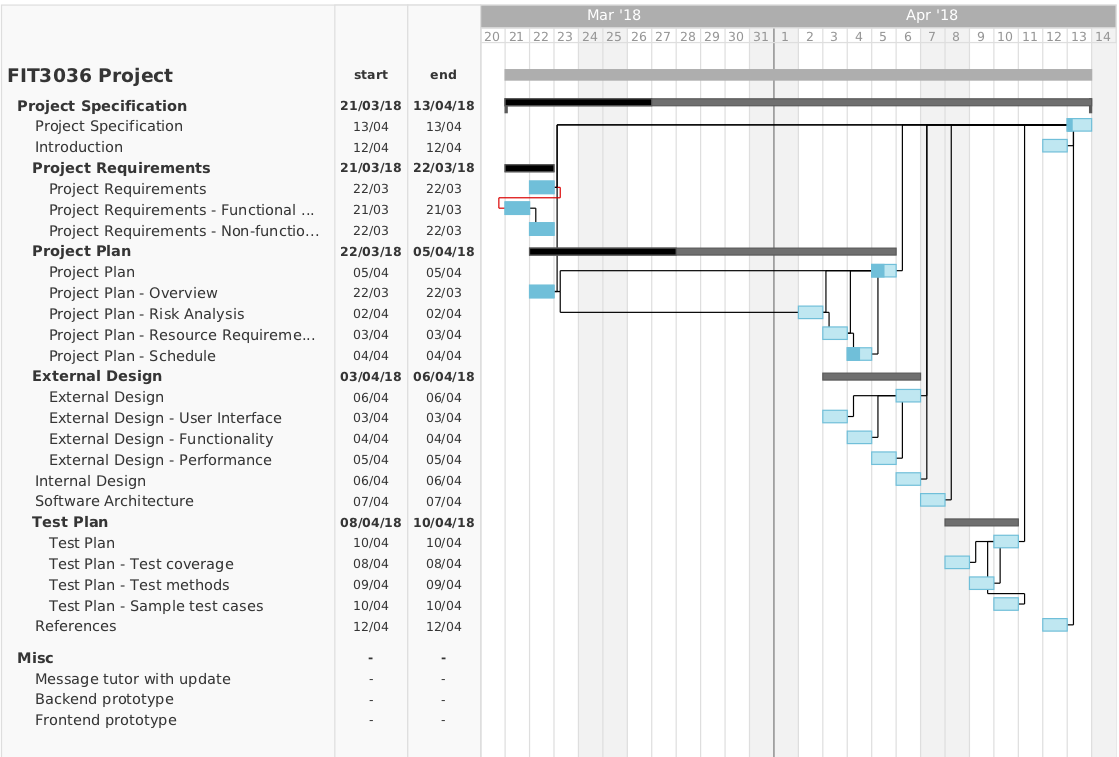
\includegraphics[width=\textwidth]{gantt-chart}
  \caption{Gantt chart}\label{fig:gantt}
\end{figure}

We also utilised Waffle \autocite{waf:20}, which connects to the multiple GitHub
repositories that hosted the code for the frontend, backend and documentation.
This allowed breaking down the large tasks into smaller ones that could be
tackled individually, this can be seen in figure~\ref{fig:waffle}.

\begin{figure}[H]
  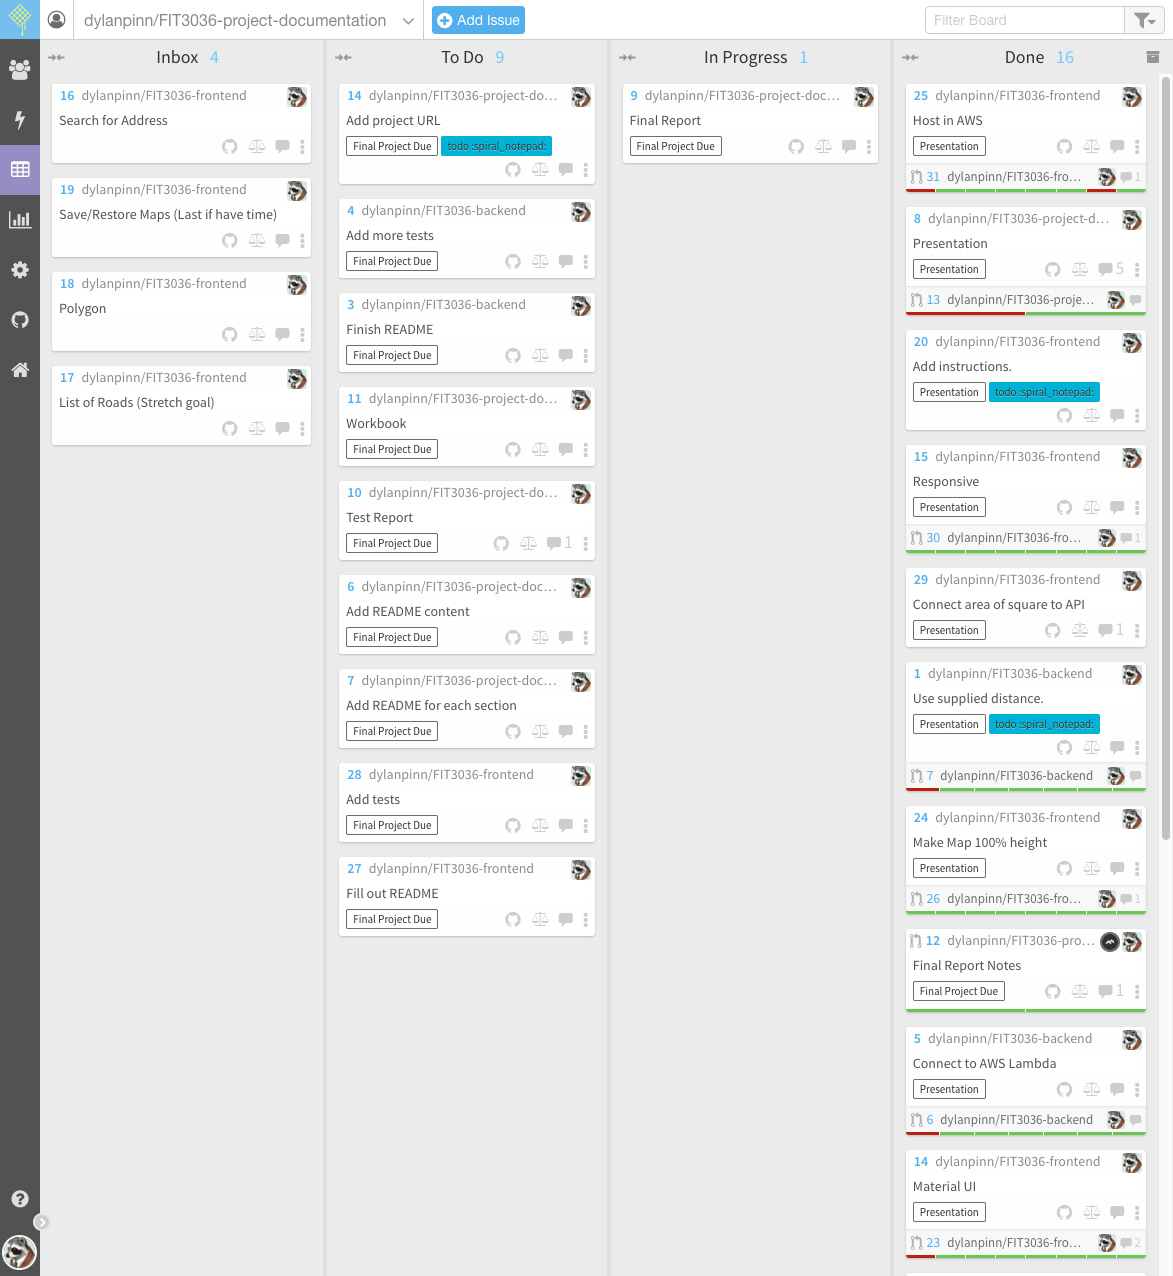
\includegraphics[width=\textwidth]{waffle-io}
  \caption{Waffle Board}\label{fig:waffle}
\end{figure}

\section{Method}

% TODO: Add intro to section.

\subsection{Methods Overview}
% TODO: Add intro to subsection.

\subsubsection{Calculate Area}
% TODO: Add intro to subsection.

\begin{itemize}
  \item The user uses the map controls in the frontend application to refine
    the desired area to calculate the surface area of the roads.
  \item The coordinates of the square is passed via a HTTP POST request to
    the backend API.\@
  \item These coordinates are used to calculate the area of the square.
  \item This is done by calculating the distance between between the
    north/south coordinates and the east/west coordinates.
  \item This is then multiplied together to return the area.
  \item This result is displayed for the user in the user interface.
\end{itemize}

\subsubsection{Calculate Surface Area of Roads}

This is the overview of how the system works to calculate the road surface area
of an area.

\begin{itemize}
  \item Once the user is satisfied with the area and clicks the ``Calculate
    Area'' button it performs a HTTP POST request to the backend API.\@
  \item The coordinates of the rectangle are sent in the POST body as JSON.\@
  \item These coordinates are used by the backend API to generate a query to
    send to OpenStreetMap via their OverPass API.\@
  \item This returns all of the road information contained within the rectangle
    bounds.
  \item The roads are then looped over, calculating the distance between each of
    the nodes of the road. Once the distance is calculated it uses the lane
    information if provided otherwise assumes that the road contains 2 lanes.
  \item The distance is multiplied by the number of lanes and the width of a
    lane, 3.5m the default lane width within Australia \autocite{lane:11}.
\end{itemize}

\subsection{Internal Design}

% TODO: Add intro to subsection.
% TODO: Add Sequence diagrams.

\paragraph{Calculate Area of a Rectangle}

% TODO: Connect to Figure.
These steps below are outlined in FIGURE

\begin{itemize}
  \item User moves the map, adjusts zoom level or changes input.
  \item The bounds of the rectangle are send to the backend service.
  \item This calculates the total area of the bounds.
  \item This is returned to the user.
\end{itemize}

\paragraph{Calculate Surface Area of Roads}

% TODO: Add Sequence diagrams.
% TODO: Connect to Figure.
These steps are outlined in FIGURE

\begin{itemize}
  \item User requests to calculate total surface area of roads.
  \item These parameters are sent to the backend service.
  \item These parameters are used to call OpenStreetMap API.\@
  \item It then iterates over the returned data and calculates the distance of
    all of the roads.
  \item If any of the points of the data are outside the bounds of the rectangle
    they are ignored.
  \item The area of the roads is then calculated with the lane width.
  \item These results are summed.
  \item This is returned to the user.
\end{itemize}

\subsection{Software Architecture}

FIGURE shows the architecture of the backend application. It is broken up into 4
main classes, which calculate area, sum data, calculate distance and calculate
the area of the roads.

% TODO: Add class diagram
% TODO: Update code or diagrams to match description.

\subsection{Algorithms}

% TODO: Add intro
% TODO: Add pseudocode for key methods.

\section{Results}

% TODO: Add intro.

The Program has 2 main outputs:

\begin{itemize}
  \item Area of the bounds.
  \item Total surface area of the road between the bounds.
\end{itemize}

The bounds is the rectangle area comprising of a set of coordinates; North,
South, East and West.

Finding reliable data to test against is hard. Writing unit tests allow testing
smaller parts of the application in isolation. This helps give confidence to the
accuracy of the application.

OpenStreetMap API returns data from outside the requested bounds. As the data
points can start within the bounds and finish outside it is excluded. This
reduces the accuracy.

Lane information isn't always included in the OpenStreetMap API so assumptions
are made about the default number of lanes. We have chose a safe default that if
no lane information is provided then the road is 2 lanes wide.

Using a default lane width of 3.5m, also reduces the accuracy. If we can find a
dataset that contains the lane width of each road with the vector data this
would help improve the accuracy of the program.

In the initial research, we couldn't find any other implementations/research
that did these calculations using vector data. Because of this the methodology
of the application was implemented through trial and error.

We created throwaway spikes to test implementation of the backend API.\@ This
included querying a small set of data and performing the calculations on it.
This helped to fine-tune and improve the accuracy of the algorithms used.

\subsection{Externally Observable Features}

% TODO: Add intro

\subsubsection{Input}

\begin{itemize}
  \item User can manipulate the Google Map component using either touch or
    mouse.
  \item User can input coordinates for the Map to centre on this position by
    using the latitude and longitude number inputs.
\end{itemize}

\subsubsection{Output}

\begin{itemize}
  \item The area in km\textsuperscript{2} of the requested area is displayed to
    the user.
  \item This is a hard-coded square of size 1km\textsuperscript{2}.
  \item The user then can request the total surface area of the roads within
    this area.
  \item This result is presented to the user in the frontend interface.
\end{itemize}

\subsection{Performance}

The backend API is hosted on AWS Lambda, this restricts the amount of time the
functions and run for and the amount of space that they can occupy.

The current restrictions are controlled in AWS, the settings are:

\begin{itemize}
  \item 1024 MB of memory.
  \item 6 seconds to run function before timing out.
\end{itemize}

\subsubsection{Area Function}

\begin{itemize}
  \item Average Invocation Time --- 3ms
  \item Average Memory Usage --- 30MB
\end{itemize}

\subsubsection{Road Surface Function}

\begin{itemize}
  \item Average Invocation Time --- 1800ms
  \item Average Memory Usage --- 28MB
\end{itemize}

\section{Analysis \& Discussion}

% TODO: Add intro

The results show that even though there are concerns about the accuracy of the
results, we were able to meet the requirements.

The performance results highlight that choosing the Go programming language
for the backend API, allows it to perform above expectations in regards to
time and memory restrictions.

% TODO: Add more to this section.

\section{Future Work}

We have found the following future work which would help to expand and improve
upon this application.

\paragraph{System Tests} We include unit tests for both the frontend and backend
applications, but no system tests. Including tests that test the whole
application as a whole, frontend and backend, will increase the confidence in
the application and will help catch regressions and issues that could occur
between the two applications.

\paragraph{Address Search} Allowing the user to search for areas using the
Google Maps Places API.\@ This will help refine and search for areas without
having to manually move the map around or know and enter the latitude and
longitude coordinates.

\paragraph{Polygon} Allowing the user to draw the area to perform the
calculations would help, as more than likely the end user wants to perform
calculations for areas that are not perfect squares. Google Maps provides a
Polygon API which would help with the implementation of this. Implementing this
would require a substantial change to the backend APIs to allow for bounds to be
a polygon and not a rectangle.

\paragraph{List Roads with Individual Areas} This would aid the user to
understand what the total surface area is composed off. Including a list of the
roads and their individual surface areas would not be a large change as all of
this data is present from the OpenStreetMap API.\@ We just need to return it
with the Road Surface Area API call and display it on the frontend for the user.

\paragraph{Save \& Restore Maps} Allowing the user to save maps and access them
later, would be important functionality if this was to be released. This would
allow users to perform multiple calculations and then at a later time restore
them to compare.

\paragraph{Share Maps} Allowing users to share maps with other users would be a
likely must requested requirement as users would need to be able to perform
calculations and then send these to other users to review.

\section{Conclusion}

% TODO: Add Conclusion

\section{Bibliography}

\printbibliography{}

\section{Appendices}

\subsection{Production \& Deployment}

\subsubsection{Frontend Application}

The code for this application is hosted in a GitHub repository
\autocite{github:13}.

\paragraph{Local Setup}

% TODO: Add this section once frontend README has been updated.

\paragraph{Deployment}

\subsubsection{Backend Application}

The code for this application is hosted in a GitHub repository
\autocite{github:14}.

\paragraph{Local Setup}

Requirements for running the application locally are:

\begin{itemize}
  \item Go programming language version 1.10 or higher \autocite{go:8}.
  \item Dep --- Go dependency management tool \autocite{dep:12}.
\end{itemize}

\noindent{}
Installation steps:

\begin{itemize}
  \item \code{dep ensure -v} --- This installs the required dependencies.
\end{itemize}

\noindent{}
Run Locally:

\begin{itemize}
  \item \code{go run local/main.go} --- This starts a local server running on
    localhost port 8080.
  \item When running the application locally it is expecting that the local copy
    of the API server is also running.
\end{itemize}

\paragraph{Deployment}

Requirements for deploying the application to production include the development
dependencies plus:

\begin{itemize}
  \item GNU Make \autocite{gnu:15}
  \item NodeJS version $\geq 6$ \autocite{node:16}
  \item Yarn package manager \autocite{yarn:17}
  \item AWS CLI \autocite{aws:18} --- API Keys need to be configured.
\end{itemize}

\noindent{}
Installation steps:

\begin{itemize}
  \item \code{yarn install} --- This installs the serverless framework required
    to deploy the application.
\end{itemize}

\noindent{}
Deploy:

\begin{itemize}
  \item \code{make deploy} --- This builds and deploys the application.
\end{itemize}

\subsection{GUI Features}

The graphical user interface has the following features:

\begin{itemize}
  \item Google Map iFrame that mirrors the functionality found on the Google
    Maps website.
  \item Latitude \& Longitude number inputs. These manually move the centre of the map
    to the desired coordinate.
  \item ``Calculate Area'' button that performs a HTTP POST request to one of the
    backend services.
  \item Can either use the map controls or the input to control the map.
  \item The centre square is automatically drawn at a 1km \textsuperscript{2}
    area around the centre of  the map.
\end{itemize}

\subsection{User Interface}

% TODO: Add screenshots

\subsection{Internal Testing}

Both frontend and backend applications contain unit tests that can be run to
ensure the correctness of them.

\subsubsection{Frontend Tests}

To run tests for the frontend application, run the following command while in
the root directory of the application:

\begin{itemize}
  \item \code{yarn test}
  \item This starts the test runner. Entering \code{a} will run all of the tests
    in the suite.
\end{itemize}

\subsubsection{Backend Tests}

To run tests for the backend application, when in the root directory of the
project run the following command:

\begin{itemize}
  \item \code{go test ./...}
\end{itemize}

\end{document}
